\chapter{Introduction}
\label{chapter:one}


Modern software systems provide configuration options to modify
both functional behavior of the system (functionality of the system) and non-functional properties of the system ( performance and memory
consumption). 
Configuration options of a software system that are relevant to users are usually referred to as
\textit{features}. All the features of a system (vector of configuration options) together defines a \textit{configuration} of a software system. The features can  take integer, decimal or string values.  An important non-functional properties is performance, because it  influences  how a user interacts with the system. 
Environmental/external factors can affect performance. For example, the performance of the software system can be better for more number of cores and greater RAM memory.  A software system is required to select and set configuration options to maximize the performance of that system. For example, say we have a software system with 10 (binary) configuration options---it results in a configuration space of size $2^{10}$ or $1024$. The user of the software system, now has to find the optimal configuration for the given task (or input) in hand. 
This problem can be tackled in two different ways: (1) exhaustively measuring performance of all possible configurations---which means running 1024 benchmark runs, and (2) use domain knowledge (assuming the user has tuned similar software system before) to find the best configuration. 
However, as the number of configuration options increase, it
becomes difficult for humans to keep track of the interactions between the configuration options. This means as the configuration space grows it is harder to either exhaustively measure performance for all possible configurations or find domain experts to confidently do so. Please note that the optimal configuration can change dramatically with different inputs (tasks) and the environment---which make domain knowledge based decision less reliable. 

This exact problem has been reported by numerous researchers from different domains.
\begin{itemize}
\item Many software systems have poorly chosen defaults [1], [2]. Hence, it is useful to seek better configurations.
\item Understanding the configuration space of software systems with large configuration spaces is challenging [3].
\item Exploring more than just a handful of configurations is usually infeasible due to long benchmarking time [4].
\end{itemize}


The problem we are trying to tackle throughout this document is: ``How can we find a set of configuration options which would \underline{maximize} the performance of a system while \underline{minimizing} the cost of search''. Here were would limit our scope of study to just the configurations options or features of a particular software system (and not its environment). While exploring the above mentioned, we produced three methods:
\begin{enumerate}
    \item The paper titled ``Faster Discovery of Faster System Configurations with Spectral Learning'' introduced a method called \what, which improved upon the methods proposed by Guo et al.~\cite{guo2013variability} and Sarkar et al.~\cite{sarkar2015cost}. This paper was published in Automated Software Engineering Journal (ASEJ). 
    
    \item The paper titled ``Using Bad Learners to find Good Configurations'' introduced a rank-based method, which improved upon the method proposed by Guo et al. and Sarkar et al. This paper was published in Foundations of Software Engineering 2017 (FSE).
    
    \item The paper titled ``Finding faster configurations using Flash'' introduce a method called Flash, which improved upon methods proposed by Guo et al.~\cite{guo2013variability}, Sarkar et al.~\cite{sarkar2015cost}, and Zuluaga et al.~\cite{zuluaga2016varepsilon}. This paper was published in IEEE Transactions on Software Engineering (TSE).
\end{enumerate}

While this has been used in just configuration of software system, in theory is not different from general optimization strategies can be applied to many different domains. My colleagues in The RAISE Labs have been using the methods proposed in this thesis (particularly FLASH) on various other domains. The preliminary results are positive.

\section{Statement of Thesis}
This dissertation advances knowledge through several contributions, and defends
the claims of the thesis. The thesis in full
below:
\begin{center}
\begin{flushleft}
    \hspace{2cm}\textbf{Effective performance optimization  of  configurable software systems only }\\
    \hspace{2cm}\textbf{requires approximate, cheaper and easy to build models.}\\
\end{flushleft}
\end{center}

This thesis proposes 3 methods to find good configurations and we endorse the Sequential Model-based Optimization. For breif summary, see the rest of the chapter. For more details, please feel free to read the whole thesis. 


\section{Clustering}
The prior work in this area~\cite{guo2013variability, sarkar2015cost} used a combination of random sampling and regression trees. However, random sampling completely disregards the presence of clusters in the configuration space. It has been shown in the literature~\cite{oh2017finding} that (1) most of the configuration options do not influence the performance, and (2) the performance curve is generally a step function. 

\begin{figure}[!htbp]
    \centering
    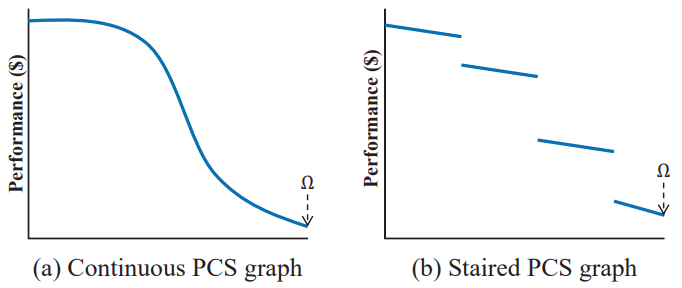
\includegraphics[width=0.8\linewidth]{Chapter-Introduction/Figures/stairs.png}
    \caption{Performance curves. (From ~\cite{oh2017finding})}
    \label{fig:chap1_stairs}
\end{figure}

To elaborate, if we sort the configurations from worst-performance to best and
plot configurations along the X-axis and performance along the
Y-axis. We expected a continuous graph
such as Figure~\ref{fig:chap1_stairs}(a), where high-valued (\$) is bad (worst performance is at the far left) and low-valued (\$) is good (best performance is at the
far right). Interestingly, Marker et al.~\cite{marker2014understanding} discovered that performance curves often occurs (in real world) as stairs, as in Figure 3b. Stairs arise from discrete feature decisions;
some features are highly-influential in performance while others
have little or no impact. Consequently, a few critical features
influences the performance while less important feature decisions alter the performance of nearby configurations only slightly (giving a stair its width and slope).

\noindent\textbf{Intuition}: From the literature, it is evident that most of the configuration options in a (given) software system does not affect the performance of the configurations. Hence, the central insight of this work is that random sampling with no regards to this specific feature of this problem is ineffective and hence adds additional cost. 

\noindent\textbf{Proposal}: This problem can be reformulated as a clustering problem, where we try to find an unsupervised method to cluster the configuration space into meaningful clusters. Once we have these clusters, we can use random samples (of configurations) from each of these clusters. This way, we can reduce redundant measurements.  

\section{Ranking}
Prior work in this area (including~\cite{nair2017faster}), tried to build accurate performance predictors, which can be used to predict the performance of a certain configuration. This work reflects on the prior work and asks: ``\textit{Our goal is to find a good configuration~\footnote{Good is defined as the distance from the optimal configuration} but, why does the prior work transform this problem into building an accurate model?}'' Another reason for this question is the very nature of the model building process previously described in Figure~\ref{fig:chap1_sampling_process}. We ask the question ``How does a user define \textit{Good}''? There is no way for the user to know whether a model can be build with MMRE less that 10\%. 

With respect to aforementioned questions, we drastically modify our approach to this problem. We hypothesize that to find the best performing configuration, we do not want a model which can return a predicted performance score which is as close to the actual performance score. Instead, we build a model which preserves the relative ordering of the configurations. 

\noindent\textbf{Intuition}: The central insight of this work is that exact performance
values (e.g., the response time of a software system) are not
required to rank configurations and to identify the optimal one. To elaborate more, let us assume that we have two humans (Adam---134cm, Billy---173cm) (analogous to configurations) and our objective is to identify the tallest person (Billy). To identify the tallest person, do we need a model which accurately predicts their height in a nano-meter scale? We can easily identify Billy even if the bad model predicted Adams height as 700cm and 890cm. 

\noindent\textbf{Proposal}: 
We show that, if we (slightly) relax the question
we ask, we can build useful predictors using very small sample sets.
Specifically, instead of asking ``How long will this configuration
run?'', we ask instead ``Will this configuration run faster than that
configuration?'' or ``Which is the fastest configuration?''.


\section{Sequential-Model Based Sampling}
Prior work in this area primarily used two strategies.
Firstly, researchers used machine learning to model the configuration
space. The model is built sequentially, where new
configurations are sampled randomly, and the quality or
accuracy of the model is measured using a holdout set. The
size of the holdout set in some cases could be up to 20\% of
the configuration space~\cite{nair2017using} and needs to be evaluated (i.e.,
measured) before even the model is fully built. This strategy
makes these methods not suitable in a practical setting since
the generated holdout set can be (very) expensive. Secondly,
the sequential model-based techniques used in prior work
relied on Gaussian Process Models (GPM) to reflect on the
configurations explored (or evaluated) so far~\cite{zuluaga2016varepsilon}. However,
GPMs do not scale well for software systems with more than
a dozen configuration options~\cite{wang2016bayesian}.



\noindent\textbf{Intuition}: 
To reduce the cost of sampling and eliminate the need for holdout set, we use sequential Model-based Optimization (SMBO). SMBO uses the Bayesian methodology to the iterative optimizer by incorporating a prior model (built using configuration which are already measured) on the space of possible target functions, $f$. By updating this model every time time a configuration is evaluated, a SMBO routine keeps a posterior model of the target function $f$. This posterior model is the surrogate $f^*$ for the function f (ground truth). Figure~\ref{fig:chap1_smbo} encapsulates the process.

\begin{figure}[!htbp]
    \centering
    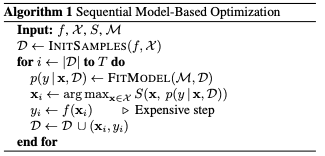
\includegraphics[width=0.6\linewidth]{Chapter-Introduction/Figures/bayesian_opt.png}
    \caption[Algorithm for SMBO methods]{Sequential Model-based Optimization. (From ~\url{http://tiny.cc/3hy80y})}
    \label{fig:chap1_smbo}
\end{figure}

\noindent\textbf{Proposal}:
We use the intuition present above to develop a method called FLASH.
The key idea of FLASH is to build a performance model
that is just accurate enough for differentiating better configurations
from the rest of the configuration space. Tolerating
the inaccuracy of the model is useful to reduce the cost
(measured in terms of the number of configurations evaluated)
and the time required to find the better configuration.
To increase the scalability of methods using GPM (Gaussian Process Models)---used widely in the machine learning domain, FLASH
replaces the GPMs with a fast and scalable decision tree learner.





\section{How to Read the Dissertation}
This dissertation is organized as self-contained chapters that together support
the thesis.

\textbf{Chapter~\ref{chapter:one}} explains, identifies and provides context for the research problem, articulates the objective, significance, and scope of the work.

\textbf{Chapter~\ref{chapter:background}} presents the background and related work in this area. The area of performance optimization has been explored not just in the domain of software engineering and has gained a lot of interest in the systems community as well. In general, there has been a considerable interest in the black-box optimization literature. In this chapter, an attempt has been made to describe the research work using the terminology used in the rest of the thesis.

\textbf{Chapter~\ref{chapter:WHAT}} describes the design and implementation
of \emph{WHAT}.
{\what}'s innovation is  
the use of the spectrum (eigenvalues) of the distance matrix
between the configurations of a configurable software system, to perform dimensionality reduction. Within that
reduced configuration space, many closely associated configurations can be studied
by executing only a few sample configurations. For the subject systems studied
here, a few dozen samples yield accurate and stable predictors---less than 10\,\% prediction error, with a standard deviation of less than 2\,\%.  
When compared to the state of the art, our approach (a)~requires 
2 to 10 times fewer samples to achieve similar prediction accuracies,
and (b)~its predictions are  more stable (i.e., have lower standard
deviation). 
Furthermore, we demonstrate that predictive models generated by
\what can be used by optimizers to discover system configurations that closely approach the optimal performance.


\textbf{Chapter~\ref{chapter:rank}} proposes using ranking models instead of regression models to save cost while finding good configurations. The central  insight of this chapter is that   
exact performance values (e.g., the response time of a software system) are not required to rank  configurations and to identify the optimal one. 
As shown by our experiments, performance models that are cheap to learn but inaccurate (with respect to the difference between actual and predicted performance) can still be used rank configurations and hence find the optimal configuration. This novel \emph{rank-based approach} allows us to significantly reduce the cost (in terms of number of measurements of sample configuration) as well as the time required to build performance models. We evaluate our approach with 21 scenarios based on 9 software systems and demonstrate that our approach is beneficial in 16 scenarios; for the remaining 5 scenarios, an accurate model can be built by using very few samples anyway, without the need for a rank-based approach.

In \textbf{Chapter~\ref{chapter:flash}}, we design and implement FLASH. The central insight of this paper is to use the prior knowledge (gained from prior runs) to choose the next promising configuration. This strategy reduces the effort (measured in terms of the number of measurements) required to find the (near) optimal configuration.  \flash can be used to solve single-objective (e.g., run-time) and can also be adapted to multi-objective (e.g., energy and runtime) performance optimization problems. 
We evaluate \flash  using 30 scenarios based on 7 software systems to demonstrate that \flash saves effort in 100\% and 80\% of cases in single-objective and multi-objective problems respectively by up to several orders of magnitude. 
% We also demonstrate how \flash is more scalable than other state of the art sequential model-based methods. 
% \textcolor{red}{TODO}
% Many design processes can be described as the exploration of options. Hence, 
% \flash can be applied to many areas.
% To demonstrate this,  we evaluate \flash, beside performance configuration optimization,  on standard search-based software engineering case studies   (release planning, process modeling, and sprint planning for agile development). 
% The superior performance
% of  \flash in these software systems, plus its better scalability and faster runtimes, makes us recommend this method XXX

In \textbf{Chapter~\ref{chapter:conclusion}}, we revisit the key contributions of this thesis and provide directions for future work.